\documentclass[12pt,twoside]{article}
\usepackage{amsmath, amssymb}
\usepackage{amsmath}
\usepackage{fancyhdr,parskip}
\usepackage[active]{srcltx}
\usepackage{amssymb}
\usepackage{amscd}
\usepackage{makeidx}
\usepackage{amsthm}
\usepackage{algorithm}
\usepackage{algpseudocode}
\usepackage{fancyhdr}
\usepackage{graphics}
\usepackage{amsmath, amssymb}
\usepackage{amsmath}
\usepackage[active]{srcltx}
\usepackage{amssymb}
\usepackage{amscd}
\usepackage{makeidx}
\usepackage[dvips]{graphicx}
\usepackage{longtable}
\usepackage{tabularx}
\usepackage[table,xcdraw]{xcolor}
\usepackage{color}
\usepackage[hidelinks]{hyperref}
\usepackage[backend=biber,style=apa]{biblatex}
\usepackage{longtable}
\usepackage{tabularx}
\usepackage[table,xcdraw]{xcolor}
\usepackage{color}
\usepackage[hidelinks]{hyperref}
\usepackage{multirow}
\usepackage{algorithm}
\usepackage{algpseudocode}
\renewcommand{\algorithmicrequire}{\textbf{Input:}}
\renewcommand{\algorithmicensure}{\textbf{Output:}}
\renewcommand{\tablename}{Tabla}
\renewcommand{\figurename}{Figura}
\renewcommand{\baselinestretch}{1}
\setcounter{page}{1}
\setlength{\textheight}{21.6cm}
\setlength{\textwidth}{14cm}
\setlength{\oddsidemargin}{1cm}
\setlength{\evensidemargin}{1cm}
\pagestyle{myheadings}
\thispagestyle{empty}
\markboth{\small{Pr\'actica 2. Luis Francisco Renteria Cedillo, Denzel Omar Vazquez Perez.}}{\small{.}}
\date{}
\begin{document}
\begin{figure}[h]
\vspace{-3cm} \hspace{-2cm} \setlength{\unitlength}{1mm}
\begin{picture}(15,25)(-10,0)

\includegraphics[width=16.5cm,height=3.5cm]{imagenes/titulo.png}
\end{picture}
\end{figure}
\vspace{0cm}
\centerline{\bf An\'alisis de Algoritmos, Sem: 2022-2, 3CV11, Pr\'actica 2, 14 de marzo de 2022}
\centerline{}
\begin{center}
\Large{\textsc{Pr\'actica 2: Complejidades temporales polinomiales y no polinomiales}}
\end{center}
\centerline{}
\centerline{\bf {Luis Francisco Renteria Cedillo, Denzel Omar Vazquez Perez.}}
\centerline{}
\centerline{$lrenteriac1400@alumno.ipn.mx, dvazquezp1600@alumno.ipn.mx$}
\newtheorem{Theorem}{\quad Theorem}[section]
\newtheorem{Definition}[Theorem]{\quad Definition}
\newtheorem{Corollary}[Theorem]{\quad Corollary}
\newtheorem{Lemma}[Theorem]{\quad Lemma}
\newtheorem{Example}[Theorem]{\quad Example}
\bigskip
\textbf{Resumen:} En la presente documento se muestra el comportamiento de algoritmos iterativos contra los recursivos evaluando cual de estos es el más eficiente y determinando por su complejidad algor\'itmica ¿C\'ual es le mejor a implementar?, por otra parte se habla de n\'umeros perfectos y sus implementaci\'on para sus posterior evaluaci\'on ante un equipo de c\'omputo convencional.\\

{\bf Palabras Clave:} Fibonacci, Numeros Perfectos, Recursividad, Complejidad, C++ .
\section{Introducci\'on}
Hoy en d\'ia la recursi\'on e iteratividad son usadas en tareas repetitivas hasta que se cumpla alguna condici\'on, sin embargo al momento de codificar se ignora cual de estos estilos de programaci\'on es la conveniente para llegar al objetivo en el menor tiempo posible.\\\\
Es importante mencionar que se tiene la respuesta ante tal pregunta y es por medio de un an\'alisis, los algoritmos tanto iterativos como recursivos deben de pasar por un an\'alisis a \textbf{priori} tanto a \textbf{posteriori} donde en uno se busca el calculo de la complejidad algor\'itmica por medio de conceptos b\'asicos aprendidos en la Unidad de aprendizaje, y el otro permite la colecci\'on de estad\'isticas del tiempo consumidos mientras se ejecuta el algoritmo, con el fin común de encontrar una funci\'on que acote el tiempo de ejecuci\'on de la tarea a realizar.\\\\
Para esta práctica se pondr\'a en comparaci\'on el tiempo de ejecuci\'on del algoritmo de la sucesi\'on de Fibonacci tanto en su representaci\'on iterativa como recursiva con el fin de evaluar cual de estas implementaciones resulta m\'as eficiente que la otra, como segunda parte del documento dar\'a b\'usqueda de n\'umeros perfectos y como la codficaci\'on y ejecuci\'on de este algoritmo puede perjudicar directamente el rendimiento del equipo de c\'omputo con el que se trabaja. 
\section{Conceptos te\'oricos}
\subsection{Sucesi\'on de Fibonacci}
Los n\'umeros de la sucesi\'on de Fibonacci fueron definidos originalmente en el siglo XIII por el matem\'atico italiano Fibonacci para modelar el crecimiento de las grandes multitudes de conejos, definió la relación de recurrencia como:
$$X_{n}~=~X_{n-1}~+~X_{n-2}$$
Los principales casos son $X_{0}=0$ y $X_{1}=1$, por tanto $X_{2}=1$, $X_{3}=2$ donde al continuar con la sucesi\'on se tendr\'a $\{3, 5, 8, 13, 21, 34, 55, 89, 144,\cdots \}$, esta formula a la no ser buena para contar a la gran poblaci\'on de conejos, resulto tener una serie de propiedades, de las cuales tiene una estrecha relaci\'on con la sucesi\'on de Lucas y el n\'umero \'aureo $(\varphi)$ cuyo valor n\'umerico es:
$$\varphi~=~\frac{1+\sqrt{5}}{2}$$
Es posible aproximarse a este ultimo al dividir dos t\'erminos consecutivos de la sucesi\'on de Fibonacci, donde en cuanto m\'as grandes son los t\'erminos, el resultado de los cocientes se acerca m\'as a $\varphi$ .\\
La soluci\'on de este problema es posible por medio de su implementación iterativa as\'i como recursiva, cuyos pseudo-c\'odigos son:\\
\textbf{Algoritmo iterativo de la sucesi\'on de Fibonacci\\}
\begin{algorithm}[H]
  \caption{Sucecion\_Fibonacci $(int~n)$}
  \begin{algorithmic}[1]
    \Require{n} 
    \Ensure{x2}
 
    \State $x1~=~1$
    \State $x2~=~0$
 
    \For{i=1 \textbf{to} i$\leq$ n}
      \State{$x2~=~x1~+x2~$};
      \State{$x1~=~x2~-x1~$};
    \EndFor
    \State{\textbf{return} $x2$}
  \end{algorithmic}
\end{algorithm}
\textbf{Algoritmo recursivo de la sucesi\'on de Fibonacci}
\begin{algorithm}[H]
  \caption{Sucecion\_Fibonacci\_R $(int~n)$}
  \begin{algorithmic}[1]
    \Require{n} 
    \Ensure{N\'umero natural}
    
    \If{n$<$2}
      \State \textbf{return} n
    \Else
        \State \textbf{return} $($Sucecion\_Fibonacci\_R $(n-1)~+~$Sucecion\_Fibonacci\_R$(n-2)$
    \EndIf
  \end{algorithmic}
\end{algorithm}


\subsection{N\'umeros perfectos}

Un n\'umero perfecto es un n\'umero que pertenece al dominio de los números enteros y cumple la condición que es igual a la suma de sus divisores. Como ejemplo, tenemos que el numero 6 tiene divisores 1, 2 y 3. Dado que la suma de 1+2+3=6, se cumple que 6 es un n\'umero perfecto.
\newline\newline
En la antigüedad, los números perfectos eran considerados superiores a los demás y se les atribuían propiedades místicas. A pesar de que no se les ha encontrado utilidad para resolver problemas matemáticos o áreas como la criptografía, siguen siendo un misterio para los matemáticos de la actualidad.
\newline\newline
Existen tres conjeturas de los números perfectos:
\begin{enumerate}
    \item Todos los números perfectos son pares ya que tienen potencia de 2 como factor.
    \item Todos los números perfectos finalizan en 6 o 8
    \item Los números perfectos son infinitos
\end{enumerate}
No obstante, ninguno de los enunciados anteriores ha sido demostrado.
\newline
Euclides propuso una formula para obtener los números perfectos:
$$(2^{n-1})\cdot(2{n} - 1) = Numero\: Perfecto$$ 
Donde n  y $(2{n} - 1)$ deben ser ambos primos.
Más adelante, el matemático Euler realizó la demostración que todos los números perfectos se generan por la fórmula propuesta por Euclides.

\subsubsection{Test de Primalidad de Fermat}
La prueba o test de primalidad de Fermat es una prueba que utiliza el pequeño teorema de Fermat y establece que si un numero primo $p$ y un numero coprimo $a$ con $p$ , entonces $a^{p-1}$ es divisible por $p$. Se describe de la siguiente forma:
$$a^{p-1} \equiv 1(mod\:p)$$
Sin embargo, existe la posibilidad de que el resultado sea un falso positivo, dado a que es un algoritmo probabilístico. Es por ello que debe ejecutarse determinado numero de veces para reducir la probabilidad de error.
\begin{algorithm}[H]
  \caption{testPrimalidadFermat$(int~n, int~iteraciones)$}
  \begin{algorithmic}[1]
    \Require{n,iteraciones} 
    \Ensure{Primo si n es un posible primo, caso contrario regresa Compuesto}
    
    \For{i=1 \textbf{to} i$\leq$ iteraciones}
      \State $a~=random_generator(1,n-1)$
    \If{$a^{n-1}\not\equiv 1(mod\:n)$}
        \State \textbf{return} Compuesto
    \EndIf
    \EndFor
    \State \textbf{return} Primo
    
  \end{algorithmic}
\end{algorithm}
\section{Experimentaci\'on y resultados}
\subsection{Algoritmos para la sucesi\'on de Fibonacci}
Este primer problema tiene dos secciones donde se encuentra tanto su soluci\'on a partir de su relaci\'on iterativa como por su relaci\'on de recurrencia, presentando un an\'alisis detallado para determinar su complejidad algor\'itmica en base a su codificaci\'on en lenguaje C.
\subsubsection{Implementaci\'on iterativa de la Sucesión de Fibonacci}
Para la implementaci\'on iterativa de los n\'umeros de Fibonacci se hace uso del \textbf{Algorithm 1} visto en la sección de \textit{Conocimientos te\'oricos}.\\[0.6cm]
\textbf{3.1.1.1 An\'alisis a priori}\\[0.4cm]
Para conocer la complejidad temporal que tiene el algoritmo sobre el espacio del tiempo, es fundamental hacer el calculo de este por medio de conceptos te\'oricos para tener como resultado una funci\'on que acote el tiempo de ejcuci\'on la soluci\'on al problema planteado. En seguida se muestra en la Tabla 1 el an\'alisis linea por linea del algoritmo del la sucesi\'on de Fibonacci con el fin de mostrar el comportamiento del mejor y peor caso.
\newline
\begin{longtable}{||c|l|c|c|c||}
    \caption{An\'alisis a priori linea por linea para el mejor y peor caso}\\
    \hline
        \multirow{2}{*}{\textbf{No.}} & \textbf{C\'odigo} & \multirow{2}{*}{\textbf{Costo}} & \multicolumn{2}{|c||}{\textbf{\# Pasos ejecutables}}\\
    \cline{2-2}\cline{4-5}
         & {Sucesion\_fibonacci $($ int n $)$} & & \textbf{Mejor caso} & \textbf{Peor caso}\\
    \hline
    \textbf{1}&{\,\,\,\,x1 = 1;}&{$C_{1}$}&{1}&{1}\\
    \hline
    \textbf{2}&{\,\,\,\,x2 = 0;}&{$C_{2}$}&{1}&{1}\\
    \hline
    \textbf{3}&{\,\,\,\,for $($ i=1; i$\leq$ n; i++ $)\{$}&{$C_{3}$}&{n}&{n}\\
    \hline
    \textbf{4}&{\,\,\,\,\,\,\,\,x2 = x1 + x2;}&{$C_{4}$}&{n-1}&{n-1}\\
    \hline
    \textbf{5}&{\,\,\,\,\,\,\,\,x1 = x2 - x1; $\}$}&{$C_{5}$}&{n-1}&{n-1}\\
    \hline
    \textbf{6}&{\,\,\,\,return x2;}&{$C_{6}$}&{1}&{1}\\
    \hline
\end{longtable}

Dado al n\'umero de pasos ejecutables para el mejor y peor caso de la Tabla 1, se identifica que no existe una diferencia para cualquiera de estos, puesto, que su crecimiento asint\'otico es igual. As\'i teniendo la informaci\'on de la anterior Tabla se forma la siguiente ecuaci\'on para conocer el orden del complejidad del algoritmo expuesto:\\[0.4cm]
$T(n)~=~C_{1}~(1)~+~C_{2}~(1)~+~C_{3}~(n)~+~C_{4}~(n-1)~+~C_{5}~(n-1)~+~C_{6}~(1)$\\
$T(n)~=~C_{1}~+~C_{2}~+~nC_{3}~+~(n-1)C_{4}~+~(n-1)C_{5}~+~C_{6}$\\
$T(n)~=~C_{1}~+~C_{2}~+~nC_{3}~+~nC_{4}~+~C_{4}~+~nC_{5}~+~C_{5}~+~C_{6}$\\
$T(n)~=~nC_{3}~+~nC_{4}~+~nC_{5}~+~C_{1}~+~C_{2}~-~C_{4}~-~C_{5}~+~C_{6}$\\
$T(n)~=~(C_{3}~+~C_{4}~+~C_{5})(n)~+~(C_{1}~+~C_{2}~-~C_{4}~-~C_{5}~+~C_{6})$\\[0.2cm]
Si $A,~B~\in~\mathbb Z$, donde $A=C_{3}~+~C_{4}~+~C_{5}$ y $B=C_{1}~+~C_{2}~-~C_{4}~-~C_{5}~+~C_{6}$, entonces $T(n)~=~A(n)~+~B~ \therefore~T(n)~\in~\Theta(n)$\\[0.5cm]
\textbf{3.1.1.2 An\'alisis a posteriori}\\[0.4cm]
Posteriormente al ejecutar funci\'on iterativa creada con el nombre \textit{"sucesion\_fibonacci"}, se tiene que el dato de entrada es un n\'umero natural (incluido el 0) $n$,  por tanto la salida del programa da el n\'umero de operaciones hechas por cada iteraci\'on, los resultados registrados se muestran en la Tabla 2.

    \begin{longtable}{||c|c||}
        \caption{Complejidad temporal de la sucesi\'on de Fibonacci iterativa}\\
            \hline
                \textbf{n}&\textbf{T(n)}\\
            \hline
                {1}&{8}\\
            \hline
                {2}&{14}\\
            \hline
                {3}&{20}\\
            \hline
                {4}&{26}\\
            \hline
                {5}&{32}\\
            \hline
                {6}&{38}\\
            \hline
                {7}&{44}\\
            \hline
                {8}&{50}\\
            \hline
                {9}&{56}\\
            \hline
                {10}&{62}\\
            \hline
                {11}&{68}\\
            \hline
                {12}&{74}\\
            \hline
    \end{longtable}
En la Figura 1 se muestra la gr\'afica obtenida para los valores de la Tabla 2.
\begin{figure}[h]
    \centering
    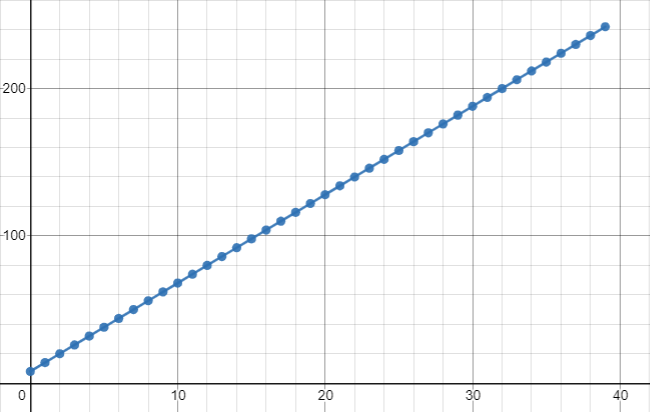
\includegraphics[width=9cm]{imagenes/grafica211.png}
    \caption{Gr\'afica del orden de complejidad del algoritmo iterativo.}
    \label{fig:my_label}
\end{figure}
Dado el comportamiento de los puntos de muestra, se aprecia que este es lineal, no habiendo diferencia entre el mejor y peor caso, y conociendo que $\Theta$ se define como:
$$\Theta(g(n)) = \{ f(n)~\arrowvert~\exists_{n}~C_{1},~C_{2}>0~\&~n_{0}>0~tal~que$$ $$0\leq~C_{1}g(n)~\leq~f(n)~\leq~C_{2}g(n)~\forall~n\geq~n_{0}\}$$
Se propone $C_{1}=4$, $C_{2}=8$ y $n_{0}=6$, es posible obsevar en la Figura 2 que dados estos valores se acotan la parte superior como la inferior as\'i como el punto de cruce en el que se cumple la inecuaci\'on, por tanto se puede decir que $T(n)\in \Theta(n)$.
\begin{figure}[H]
    \centering
    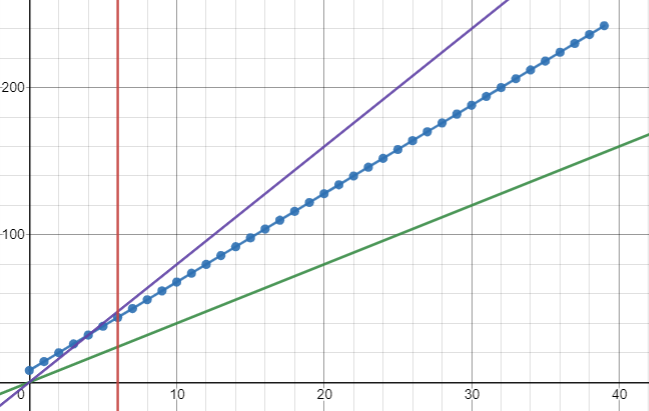
\includegraphics[width=9cm]{imagenes/grafica212.png}
    \caption{Gr\'afica de las curvas que acotan en la parte superior e inferior a los puntos mu\'estrales}
    \label{fig:my_label}
\end{figure}
\subsubsection{Implementaci\'on recursiva de la Sucesión de Fibonacci}
Posteriormente al ejecutar funci\'on recursiva creada con el nombre \textit{"sucesion\_fibonacci\_R"}, se tiene que el dato de entrada es un n\'umero natural (incluido el 0) $n$,  por tanto la salida del programa da el n\'umero de operaciones hechas, los resultados registrados se muestran en la Tabla 3.
\begin{longtable}{||c|c||}
        \caption{Complejidad temporal de la sucesi\'on de Fibonacci recursiva}\\
            \hline
                \textbf{n}&\textbf{T(n)}\\
            \hline
                {1}&{2}\\
            \hline
                {2}&{2}\\
            \hline
                {3}&{8}\\
            \hline
                {4}&{14}\\
            \hline
                {5}&{26}\\
            \hline
                {6}&{44}\\
            \hline
                {7}&{74}\\
            \hline
                {8}&{122}\\
            \hline
                {9}&{200}\\
            \hline
                {10}&{326}\\
            \hline
                {11}&{530}\\
            \hline
                {12}&{860}\\
            \hline
    \end{longtable}
Dados los tiempos de ejecución por la entrada n del algoritmo recursivo presentado se muestra que la construcci\'on hacia la soluci\'on del problema es por medio de un \'arbol, simplemente se observa que a medida que se meten valores m\'as grandes las hojas de este crecen en un ritmo exponencial, donde el tiempo de ejecuci\'on esta determinado por el siguiente cociente $\frac{X_{n+1}}{X_{n}}$ lo cual recuerda la estrecha relaci\'on que tiene la sucesi\'on de Fibonacci con el n\'umero \'aureo, por lo que para encontrar $sucesion\_fibonacci\_R(n)$ conlleva un tiempo mayor o igual que $\varphi^{n}$.\\
En la Figura 3 se muestran la cota superior e inferior donde al no a ver diferencias entre el mejor y el peor caso se hace usos de la definici\'on de $\theta$ por lo que proponiendo $C_{1}=1$, $C_{2}=2$ y $n_{0}=5$ por tanto se puede decir que $T(n)\in \Theta(\varphi^{n})$ por lo que el algoritmo presenta una complejidad exponencial.

\begin{figure}[H]
    \centering
    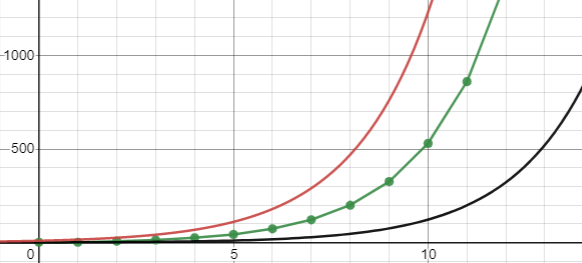
\includegraphics[width=12cm]{imagenes/grafica221.png}
    \caption{Gr\'afica de las curvas que acotan en la parte superior e inferior a los puntos mu\'estrales}
    \label{fig:my_label}
\end{figure}    

\newpage

\subsection{Algoritmo para obtener los primeros n números perfectos}
En cuanto al segundo problema, implementaremos el algoritmo de test de primalidad de Fermat, además, haremos uso del teorema de Euclides-Euler. A continuación mostraremos el análisis a priori y posteriori.
\newline
\subsubsection{An\'alisis a priori}
Para el análisis a priori, primero debemos calcular el orden de complejidad de cada linea de nuestro código. A continuación se mostraran las tablas de las funciones MostrarPerfectos(), Fermat() y Modulo().
\begin{longtable}{||c|l|c|c|c||}
    \caption{An\'alisis a priori linea por linea para el mejor y peor caso}\\
    \hline
        \multirow{2}{*}{\textbf{No.}} & \textbf{C\'odigo} & \multirow{2}{*}{\textbf{Costo}} & \multicolumn{2}{|c||}{\textbf{\# Pasos ejecutables}}\\
    \cline{2-2}\cline{4-5}
         & {modulo(int base, int e, int   mod)} & & \textbf{Mejor caso} & \textbf{Peor caso}\\
    \hline
    \textbf{1}&{\,\,\,\,a = 1;}&{$C_{1}$}&{1}&{1}\\
    \hline
    \textbf{2}&{\,\,\,\,b = base;}&{$C_{2}$}&{1}&{1}\\
    \hline
    \textbf{3}&{\,\,\,\,while$(e\textgreater{}0)\{$}&{$C_{3}$}&{$log_2(2n)+1$}&{$log_2(2n)+1$}\\
    \hline
    \textbf{4}&{\,\,\,\,\,\,\,\,if(e\%2 == 1):}&{$C_{4}$}&{$log_2(2n)$}&{$log_2(2n)$}\\
    \hline
    \textbf{5}&{\,\,\,\,\,\,\,\,\,\,\,\,a=(a*b)\%mod $\}$}&{$C_{5}$}&{$log_2(2n)$}&{$log_2(2n)$}\\
    \hline
    \textbf{6}&{\,\,\,\,\,\,\,\,b=(b*b)\%mod}&{$C_{6}$}&{$log_2(2n)$}&{$log_2(2n)$}\\
    \hline
    \textbf{7}&{\,\,\,\,\,\,\,\,e=e/2$\}$}&{$C_{7}$}&{$log_2(2n)$}&{$log_2(2n)$}\\
    \hline
    \textbf{8}&{\,\,\,\,return\:a\%mod}&{$C_{8}$}&{1}&{1}\\
    \hline
\end{longtable}

$T(n)~=~C_{1}(1)~+~C_{2}(1)~+~C_{3}(log_2(2n)+1)~+~C_{4}(log_2(2n))~+~C_{5}(log_2(2n))~+~\\C_{6}(log_2(2n))+~C_{7}(log_2(2n))+~C_{8}(1)$\\

$T(n)~=~C_{1}~+~C_{2}~+~C_{3}(log_2(2n))~+~C_{3}~+~C_{4}(log_2(2n))~+~C_{5}(log_2(2n))~+~\\C_{6}(log_2(2n))+~C_{7}(log_2(2n))+~C_{8}$\\

$T(n)~=~C_{1}~+~C_{2}~+~C_{3}~+~C_{8}+~C_{3}(log_2(2n))~+~C_{4}(log_2(2n))~+~C_{5}(log_2(2n))~+~\\C_{6}(log_2(2n))+~C_{7}(log_2(2n))$\\

Si $A,~B~\in~\mathbb Z$, donde $A=C_{3}~+C_{4}~+C_{5}~+C_{6}~+C_{7}~$ y $B=C_{1}~+~C_{2}~+~C_{3}+~C_{8}$ y , entonces $T(n)~=~A(log_2(n))~+~B~ \therefore~T(n)~\in~\Theta(log_2(n))$\\

\newpage
\begin{longtable}{||c|l|c|c|c||}
    \caption{An\'alisis a priori linea por linea para el mejor y peor caso de la funci\'on Fermat}\\
    \hline
        \multirow{2}{*}{\textbf{No.}} & \textbf{C\'odigo} & \multirow{2}{*}{\textbf{Costo}} & \multicolumn{2}{|c||}{\textbf{\# Pasos ejecutables}}\\
    \cline{2-2}\cline{4-5}
         & {modulo(int base, int e, int   mod)} & & \textbf{Mejor caso} & \textbf{Peor caso}\\
    \hline
    \textbf{1}&{\,\,\,\,if$(m==1)$}&{$C_{1}$}&{1}&{1}\\
    \hline
    \textbf{2}&{\,\,\,\,\,\,\,\,return false}&{$C_{2}$}&{1}&{1}\\
    \hline
    \textbf{3}&{\,\,\,\,for$(int j=0;j<20;j++)\{$}&{$C_{3}$}&{21}&{21}\\
    \hline
    \textbf{4}&{\,\,\,\,\,\,\,\,$x = rand() \% (m-1) +1 $}&{$C_{4}$}&{$20log_2(2n)$}&{$20log_2(2n)$}\\
    \hline
    \textbf{5}&{\,\,\,\,\,\,\,\,if(modulo(x,m-1,m)$\}$}&{$C_{5}$}&{$20log_2(2n)$}&{$20log_2(2n)$}\\
    \hline
    \textbf{6}&{\,\,\,\,\,\,\,\,\,\,\,\,return false$\}$}&{$C_{6}$}&{$20log_2(2n)$}&{$20log_2(2n)$}\\
    \hline
    \textbf{7}&{\,\,\,\,return true}&{$C_{7}$}&{1}&{1}\\
    \hline
\end{longtable}

$T(n)~=~C_{1}(1)~+~C_{2}(1)~+~C_{3}(21)~+~C_{4}(20log_2(n))~+~C_{5}(20log_2(n))~+~C_{6}(20log_2(n))+~C_{7}(1)$\\
$T(n)~=~C_{1}~+~C_{2}~+~C_{3}~+~C_{4}+~C_{7}+~C_{4}(log_2(n))~+~C_{5}(log_2(n))+~C_{6}(log_2(n))$\\
Si $A,~B~\in~\mathbb Z$, donde $A=C_{1}~+C_{2}~+C_{3}~+C_{4}~+C_{7}~$ y $B=C_{1}~+~C_{4}~+~C_{5}+~C_{6}$ y , entonces $T(n)~=~A(log_2(n))~+~B~ \therefore~T(n)~\in~\Theta(log_2(n))$\\


\begin{longtable}{||c|l|c|c|c||}
    \caption{An\'alisis a priori linea por linea para el mejor y peor caso de la funci\'on Mostrar Perfectos}\\
    \hline
        \multirow{2}{*}{\textbf{No.}} & \textbf{C\'odigo} & \multirow{2}{*}{\textbf{Costo}} & \multicolumn{2}{|c||}{\textbf{\# Pasos ejecutables}}\\
    \cline{2-2}\cline{4-5}
         & {mostrarPerfectos(int n)} & & \textbf{Mejor caso} & \textbf{Peor caso}\\
    \hline
    \textbf{1}&{\,\,\,\,i = 1}&{$C_{1}$}&{1}&{1}\\
    \hline
    \textbf{2}&{\,\,\,\,while(n)}&{$C_{2}$}&{1}&{1}\\
    \hline
    \textbf{3}&{\,\,\,\,if $(Fermat(i)==1)$}&{$C_{3}$}&{$log_2(2n)$}&{$log_2(2n)$}\\
    \hline
    \textbf{4}&{\,\,\,\,\,\,\,\,if $(Fermat(2^{i-1})\{$}&{$C_{4}$}&{$log_2^2(2n)$}&{$log_2^2(2n)$}\\
    \hline
    \textbf{5}&{\,\,\,\,\,\,\,\,\,\,\,\,Mostrar $(2^{i-1})\cdot(2^i-1)$ es perfecto}&{$C_{5}$}&{$log_2^2(2n)$}&{$log_2^2(2n)$}\\
    \hline
    \textbf{6}&{\,\,\,\,\,\,\,\,\,\,\,\,n--$\}$}&{$C_{6}$}&{$log_2^2(2n)$}&{$log_2^2(2n)$}\\
    \hline
    \textbf{7}&{\,\,\,\,\,\,\,\,i++}&{$C_{7}$}&{$log_2(2n)$}&{$log_2(2n)$}\\
    \hline
\end{longtable}

$T(n)~=~C_{1}(1)~+~C_{2}(1)~+~C_{3}(log_2(n))~+~C_{4}(log_2^2(n))~+~C_{5}(log_2^2(n))~+~C_{6}(log_2^2(n))+~C_{7}(log_2(n))$\\
$T(n)~=~C_{1}~+~C_{2}~+(~C_{3}~+~C_{7})\cdot(log_2(2n)+(~C_{4}~+~C_{5}+~C_{6})\cdot(log_2^2(2n))$\\
Si $A,~B~,~C~\in~\mathbb Z$, donde $A=C_{4}~+C_{5}~+C_{6}~$ , $B=C_{3}~+~C_{7}~$ y $C=C{1}+C{2}$ , entonces $T(n)~=~A(log_2^2(n))~+~B(log_2(n)~+C \therefore~T(n)~\in~\Theta(log_2^2(n))$\\

\newpage
\subsubsection{An\'alisis a posteriori}
En nuestro análisis a posteriori podremos identificar el numero de ejecuciones del código por cada incremento en n, siendo n los primeros números perfectos.
\newline
A continuación se mostrará la tabla de los primeros ocho números perfectos y su respectivo numero de ejecuciones para obtenerlo.

\begin{longtable}{||c|c||}
        \caption{Complejidad temporal de MostrarPerfectos()}\\
            \hline
                \textbf{n}&\textbf{T(n)}\\
            \hline
                {1}&{478}\\
            \hline
                {2}&{1088}\\
            \hline
                {3}&{1936}\\
            \hline
                {4}&{2967}\\
            \hline
                {5}&{5067}\\
            \hline
                {6}&{7095}\\
            \hline
                {7}&{9212}\\
            \hline
                {8}&{13770}\\
            \hline
\end{longtable}
Como puede apreciarse en la figura 4, el comportamiento de nuestro algoritmo pertenece a una ecuación cuadrática que se aproxima a $220n^2$. Sabemos que no existe diferencia entre el mejor y peor caso, y conociendo que $\Theta$ se define como:
$$\Theta(g(n)) = \{ f(n)~\arrowvert~\exists_{n}~C_{1},~C_{2}>0~\&~n_{0}>0~tal~que$$ $$0\leq~C_{1}g(n)~\leq~f(n)~\leq~C_{2}g(n)~\forall~n\geq~n_{0}\}$$
Se propone $C_{1}=100$, $C_{2}=300$ y $n_{0}=4$, y con estos valores la cota superior es de $300n^2$, mientras que la cota inferior es de $100n^2$.Observamos que tanto las cotas como el punto de cruce cumplen la inecuaci\'on, por tanto se puede decir que $T(n)=220n^2 \in \Theta(n^2)$.


\begin{figure}[h]
    \centering
    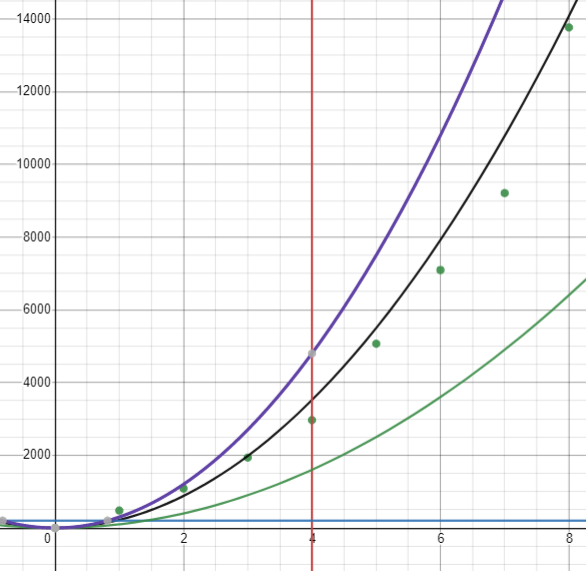
\includegraphics[width=8cm]{imagenes/grafica2-2a.png}
    \caption{Gr\'afica de las curvas que acotan en la parte superior e inferior a los puntos mu\'estrales}
    \label{fig:my_label}
\end{figure}  

La Figura 5 muestra la salida de la ejecución del código. Se alcanzaron hasta ocho números en un tiempo de 0.16 segundos, el cual es un tiempo muy razonable. Sin embargo el noveno numero tarda más de 2 minutos en encontrarlo. Podemos ver que a partir del cuarto numero, las cantidades se vuelven exponenciales, tan solo el octavo numero ya cuenta con 19 dígitos.

\begin{figure}[h]
    \centering
    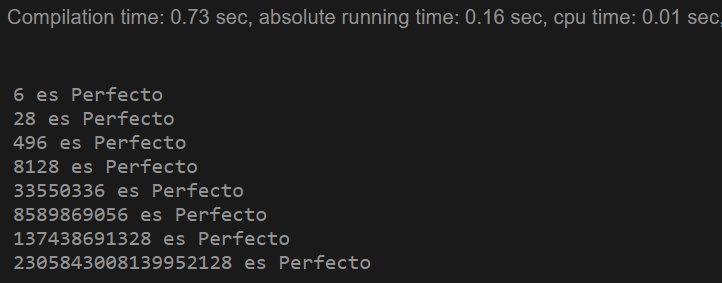
\includegraphics[width=10cm]{imagenes/salida2-2a.png}
    \caption{Salida de la ejecución del programa}
    \label{fig:my_label}
\end{figure}  

\clearpage
\newpage


\section{Conclusiones}
\textbf{\large Luis Francisco Renteria Cedillo}
\begin{figure}[H]
    \centering
    
\includegraphics[angle=0, scale=0.5]{imagenes/foto1.png}
\end{figure}

En esta practica se pudo verificar la importancia de desarrollar algoritmos eficientes, ya que, en el segundo problema, el código hecho por fuerza bruta tardaba demasiado y no llegaba a mostrar más de cuatro números perfectos en un tiempo menor a treinta segundos. Investigando más sobre estos números, encontramos la formula de Euclides, y solo debíamos encontrar los primos que cumplían sus condiciones. Aquí fue cuando recordé el teorema de Fermat y su algoritmo de test de primalidad, el cual es probabilístico y debe ejecutarse varias veces para reducir su probabilidad de falsos positivos. Dicho algoritmo lo usamos en la asignatura de criptografía, en específico al desarrollar el sistema de encriptado RSA. Con esto se pudo lograr alcanzar los primeros ocho números perfectos.

\textbf{\large Denzel Omar Vazquez Perez}
\begin{figure}[H]
    \centering
    
\includegraphics[angle=-90, scale= 0.05]{imagenes/foto2.jpg}
\end{figure}
Una de las cosas que deja de aprendizaje la practica es de nuevo que el estilo de programaci\'on afecta directamente en los resultados que se espera obtener, esto se logra percatar en el el algoritmo de los n\'umeros de Fibonacci donde la implementación iterativa como recursiva afecta directamente en el tiempo de ejecuci\'on de tal programa ya que la meter un n mas grande el proceso y los plazos de tiempo se hacen mas grandes esto es evidente en el algoritmo recursivo puesto que su complejidad es exponencial mientras que la del algoritmo iterativo es  lineal.\\
Para el segundo problema la primer implementaci\'on se hizo en C sin embargo el tiempo de espera por la ejecuci\'on es inmenso por lo que se decidio codificar en C++, para obtener un resultado mas amplio a partir de conceptos matem\'aticos un poco mas avanzados, as\'i se logro mostrar de manera eficiente los n\'umeros perfectos que se solicitaban en la practica. Sin embargo es interesante observar que es importante el tener una noci\'on del algoritmo a usar ya que dada su complejidad sera la forma mas r\'apida de resolver el problema.


\section{Bibliograf\'ia}

Wolfram Research (2022) \textit{Perfect Numbers}, disponible en\\
https://mathworld.wolfram.com/PerfectNumber.html, consultado el 14 de marzo del 2022.\\[0.4cm]
Brassard, G. (1997). \textit {Fundamentos de Algoritmia}. España: Ed. Prentice Hall.\\[0.4cm]
Cormen, E. A. (2022). \textit{Introduction To Algorithms}, 3Rd Ed. Phi.\\[0.4cm]
Luna, Benjam\'in. \textit{Fundamentos para el an\'alisis de eficiencia algor\'itmica}. Escuela Superior de Computo, IPN. M\'exico. 14 de Marzo de 2022.\\[0.4cm]
S\'anchez, P. J. I. (2006). \textit{Análisis y diseño de algoritmos: un enfoque teórico y práctico}. Servicio de Publicaciones y Divulgación Científica de la UMA.


\end{document}
